\documentclass[10pt, t]{beamer}
\usetheme{metropolis}           % Use metropolis theme

\ifnotes
  \hypersetup{final}
  \usepackage{pgfpages}
  \setbeamertemplate{note page}[plain]
  \setbeameroption{show notes on second screen=right}
\fi

\usepackage{appendixnumberbeamer}
\usepackage{multicol}
\usepackage{multirow}
\usepackage{verbatim}
\usepackage{tikz}
\usetikzlibrary{decorations.pathreplacing}
\usepackage[scale=3]{ccicons}   % creative commons icons

\title{Computer organization}
\date{}
\author{Jeremy Iverson}
\institute{College of Saint Benedict \& Saint John's University}
\begin{document}
  \maketitle

  \begin{frame}{plan for the day}
    \begin{itemize}
      \item computer organization
        \begin{itemize}
          \item central processing unit
          \item main memory
          \item cache memory
        \end{itemize}
      \item case study: matrix multiplication
      \item using Git
      \item \texttt{printf("hello, world\textbackslash n");}
    \end{itemize}
  \end{frame}

  \begin{frame}[standout]
    central processing unit (CPU)

    \note{activity with Pep/9 ISA\\}
  \end{frame}

  \begin{frame}[standout]
    what does memory look like?

    \note{have students draw a picture of ``memory''\\}
  \end{frame}

  \begin{frame}{memory organization}
    \setlength{\columnsep}{-2.5cm}
    \begin{multicols}{2}
        \vspace{3ex}
        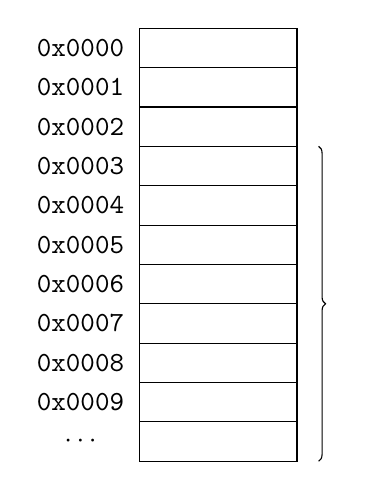
\begin{tikzpicture}
          \foreach \y in {0,0.5,...,5}
            \draw (-.75,\y) rectangle ++(2,.5);

          \uncover<2->{
            \foreach \y in {0,...,9}
              \node at (-1.5,5.25-.5*\y) {\texttt{0x000\y}};
            \node at (-1.5,.25) {$\boldsymbol{\cdots}$};
          }

          \uncover<3->{
            \draw[decoration={brace,raise=-5pt,mirror},decorate] (1.7,0) --
              node[right] {} ++(0,4);
          }
        \end{tikzpicture}

        \columnbreak

        \begin{itemize}
          \item<1-> memory is organized sequentially
          \item<2-> memory is addressed starting from the \emph{top}
            \begin{itemize}
              \item granularity is a byte
            \end{itemize}
          \item<3-> a process and its data can be stored anywhere in memory
            \begin{itemize}
              \item<4-> physical vs. logical addressing
              \item<5-> each process has its own \emph{address space}
            \end{itemize}
        \end{itemize}
    \end{multicols}

    \note{
      \begin{itemize}
        \item a process is an instance of a computer program
        \item a multitasking operating system is capable of running many
          processes despite having only one or a ``small'' number of physical
          cores
          \begin{itemize}
            \item context switches the processes at predefined time slices
            \item \texttt{top} activity
          \end{itemize}
      \end{itemize}
    }
  \end{frame}

  \begin{frame}{cache memory}
    \begin{itemize}
      \item \only<1>{what is it?}\only<2->{a high-speed memory co-located with
        the CPU on the chip}
      \item<3-> \only<3>{what problem is cache addressing?}\only<4->{CPU can
        compute faster than memory can be fetched
          \begin{itemize}
            \item many problems reuse data or use data that is stored near each
              other in memory, known as \emph{temporal} and \emph{spatial}
              locality, respectively
          \end{itemize}
        }
      \item<5-> \only<5>{how does it work?}\only<6->{when memory load is issued,
        cache is checked to see if the data exists there. if not, it is loaded
        from main memory and stored in cache. when cache becomes full, old data
        is evicted to make room for new.}
      \item<7-> \only<7>{how much is there?}\only<8->{multiple levels of cache,
        each larger than the previous, but all much smaller than main memory}
    \end{itemize}

    \note{
      \begin{itemize}
        \item \texttt{lscpu}
        \item \texttt{cat /proc/cpuinfo} activity for CPU info
        \item \texttt{cat /sys/devices/system/cpu/cpu0/cache/} for cache info
        \item L1, L2, L3
          \begin{itemize}
            \item L1 is usually split into data and instruction
            \item L2 is usually not shared, i.e., each core has its own
            \item L3 is usually shared by multiple cores
          \end{itemize}
      \end{itemize}
    }
  \end{frame}

  \begin{frame}[fragile]{cache performance}
    From Intel Performance Analysis Guide:
    \begin{tiny}
      \begin{verbatim}
        Core i7 Xeon 5500 Series Data Source Latency (approximate)               [Pg. 22]

        local  L1 CACHE hit,                              ~4 cycles (   2.1 -  1.2 ns )
        local  L2 CACHE hit,                             ~10 cycles (   5.3 -  3.0 ns )
        local  L3 CACHE hit, line unshared               ~40 cycles (  21.4 - 12.0 ns )
        local  L3 CACHE hit, shared line in another core ~65 cycles (  34.8 - 19.5 ns )
        local  L3 CACHE hit, modified in another core    ~75 cycles (  40.2 - 22.5 ns )

        remote L3 CACHE (Ref: Fig.1 [Pg. 5])        ~100-300 cycles ( 160.7 - 30.0 ns )

        local  DRAM                                                   ~60 ns
        remote DRAM                                                  ~100 ns
      \end{verbatim}
    \end{tiny}
  \end{frame}

  \begin{frame}{more about latency}
    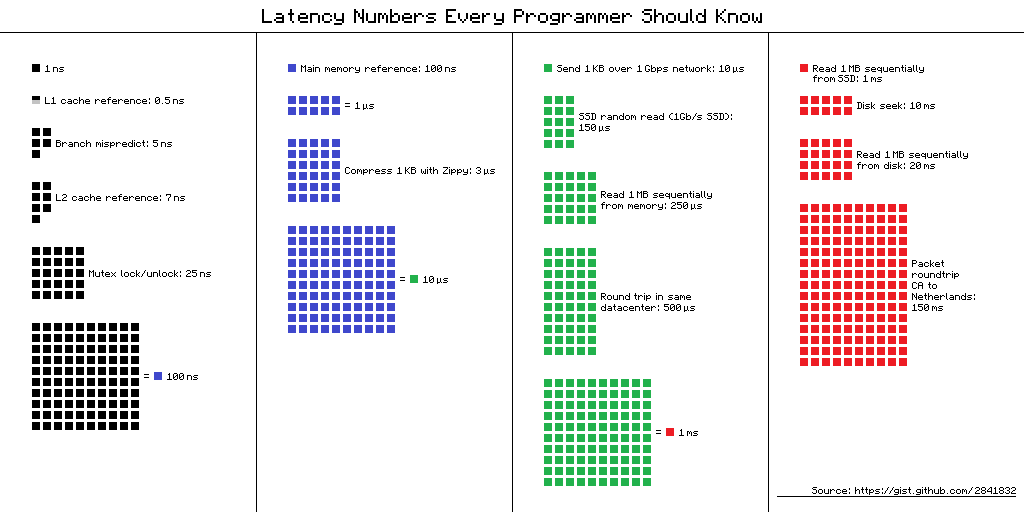
\includegraphics[width=\textwidth]{cache-perf.png}\\
    \hfill \tiny{\href{https://i.stack.imgur.com/a7jWu.png}{Latency Numbers
    Every Programmer Should Know}}
  \end{frame}

  \appendix

  \begin{frame}[c]
    \begin{center}\ccbysa\end{center}

    except where otherwise noted, this worked is licensed under
    \href{http://creativecommons.org/licenses/by-sa/4.0/}{creative commons
    attribution-sharealike 4.0 international license}
  \end{frame}
\end{document}
